\documentclass[journal,12pt,twocolumn]{IEEEtran}
\usepackage{setspace}
\usepackage{gensymb}
\singlespacing
\usepackage[cmex10]{amsmath}

\usepackage{relsize}
\usepackage{amsthm}
\usepackage{hyperref}
\hypersetup{
    colorlinks=true,
    linkcolor=blue,
    filecolor=magenta,      
    urlcolor=cyan,
}
\urlstyle{same}
\usepackage{placeins}
\usepackage{newtxtext}
\usepackage{mathrsfs}
\usepackage{txfonts}
\usepackage{stfloats}
\usepackage{bm}
\usepackage{cite}
\usepackage{cases}
\usepackage{subfig}
\usepackage{longtable}
\usepackage{multirow}
\usepackage{enumitem}
\usepackage{mathtools}
\usepackage{steinmetz}
\usepackage{tikz}
\usepackage{circuitikz}
\usepackage{verbatim}
\usepackage{tfrupee}
\usepackage[breaklinks=true]{hyperref}
\usepackage{booktabs}
\usepackage{graphicx}
\usepackage{tkz-euclide}
\usetikzlibrary{shapes,backgrounds}
\usepackage{verbatim}
\usetikzlibrary{calc,math,matrix}
\usepackage{listings}
    \usepackage{color}                                            %%
    \usepackage{array}                                            %%
    \usepackage{longtable}                                        %%
    \usepackage{calc}                                             %%
    \usepackage{multirow}                                         %%
    \usepackage{hhline}                                           %%
    \usepackage{ifthen}                                           %%
    \usepackage{lscape}     
\usepackage{multicol}
\usepackage{chngcntr}
\usepackage{mdframed}
\DeclareMathOperator*{\Res}{Res}

\renewcommand\thesection{\arabic{section}}
\renewcommand\thesubsection{\thesection.\arabic{subsection}}
\renewcommand\thesubsubsection{\thesubsection.\arabic{subsubsection}}

\renewcommand\thesectiondis{\arabic{section}}
\renewcommand\thesubsectiondis{\thesectiondis.\arabic{subsection}}
\renewcommand\thesubsubsectiondis{\thesubsectiondis.\arabic{subsubsection}}


\hyphenation{op-tical net-works semi-conduc-tor}
\def\inputGnumericTable{}                                 %%

\lstset{
%language=C,
frame=single, 
breaklines=true,
columns=fullflexible
}

\tikzset{ 
table/.style={
  matrix of math nodes,
  row sep=-\pgflinewidth,
  column sep=-\pgflinewidth,
  nodes={rectangle,draw=black,text width=3.3em,align=center},
  text depth=0.25ex,
  text height=2ex,
  nodes in empty cells
  }
}

\usepackage{chngcntr}
\counterwithin{figure}{section}

\title{AI1103 \\ Assignment 4}
\author{Nagubandi Krishna Sai \\ MS20BTECH11014}

\begin{document}
\newtheorem{theorem}{Theorem}[section]
\newtheorem{problem}{Problem}
\newtheorem{proposition}{Proposition}[section]
\newtheorem{lemma}{Lemma}[section]
\newtheorem{corollary}[theorem]{Corollary}
\newtheorem{example}{Example}[section]
\newtheorem{definition}[problem]{Definition}

\newcommand{\BEQA}{\begin{eqnarray}}
\newcommand{\EEQA}{\end{eqnarray}}
\newcommand{\define}{\stackrel{\triangle}{=}}
\bibliographystyle{IEEEtran}
\raggedbottom
\setlength{\parindent}{0pt}
\providecommand{\mbf}{\mathbf}
\providecommand{\pr}[1]{\ensuremath{\Pr\left(#1\right)}}
\providecommand{\qfunc}[1]{\ensuremath{Q\left(#1\right)}}
\providecommand{\sbrak}[1]{\ensuremath{{}\left[#1\right]}}
\providecommand{\lsbrak}[1]{\ensuremath{{}\left[#1\right.}}
\providecommand{\rsbrak}[1]{\ensuremath{{}\left.#1\right]}}
\providecommand{\brak}[1]{\ensuremath{\left(#1\right)}}
\providecommand{\lbrak}[1]{\ensuremath{\left(#1\right.}}
\providecommand{\rbrak}[1]{\ensuremath{\left.#1\right)}}
\providecommand{\cbrak}[1]{\ensuremath{\left\{#1\right\}}}
\providecommand{\lcbrak}[1]{\ensuremath{\left\{#1\right.}}
\providecommand{\rcbrak}[1]{\ensuremath{\left.#1\right\}}}
\theoremstyle{remark}
\newtheorem{rem}{Remark}
\newcommand{\sgn}{\mathop{\mathrm{sgn}}}
\providecommand{\abs}[1]{\vert#1\vert}
\providecommand{\res}[1]{\Res\displaylimits_{#1}} 
\providecommand{\norm}[1]{\lVert#1\rVert}
%\providecommand{\norm}[1]{\lVert#1\rVert}
\providecommand{\mtx}[1]{\mathbf{#1}}
\providecommand{\mean}[1]{E[ #1 ]}
\providecommand{\fourier}{\overset{\mathcal{F}}{ \rightleftharpoons}}
%\providecommand{\hilbert}{\overset{\mathcal{H}}{ \rightleftharpoons}}
\providecommand{\system}{\overset{\mathcal{H}}{ \longleftrightarrow}}
	%\newcommand{\solution}[2]{\textbf{Solution:}{#1}}
\newcommand{\solution}{\noindent \textbf{Solution: }}
\newcommand{\cosec}{\,\text{cosec}\,}
\providecommand{\dec}[2]{\ensuremath{\overset{#1}{\underset{#2}{\gtrless}}}}
\newcommand{\myvec}[1]{\ensuremath{\begin{pmatrix}#1\end{pmatrix}}}
\newcommand{\mydet}[1]{\ensuremath{\begin{vmatrix}#1\end{vmatrix}}}
\numberwithin{equation}{subsection}
\makeatletter
\@addtoreset{figure}{problem}
\makeatother
\let\StandardTheFigure\thefigure
\let\vec\mathbf
\renewcommand{\thefigure}{\theproblem}
\def\putbox#1#2#3{\makebox[0in][l]{\makebox[#1][l]{}\raisebox{\baselineskip}[0in][0in]{\raisebox{#2}[0in][0in]{#3}}}}
     \def\rightbox#1{\makebox[0in][r]{#1}}
     \def\centbox#1{\makebox[0in]{#1}}
     \def\topbox#1{\raisebox{-\baselineskip}[0in][0in]{#1}}
     \def\midbox#1{\raisebox{-0.5\baselineskip}[0in][0in]{#1}}
\vspace{3cm}
\title{AI1103 \\ Assignment 4}
\author{Nagubandi Krishna Sai \\ MS20BTECH11014}
\maketitle
\newpage
\bigskip
\renewcommand{\thefigure}{\theenumi}
\renewcommand{\thetable}{\theenumi}
\begin{mdframed}
Download Python code and LaTex from below link : \\
\href{https://github.com/KRISHNASAI1105/demo/tree/main/Assignment}{https://github.com/KRISHNASAI1105
/demo/tree/main/Assignment4}
\end{mdframed}
\subsection*{\boldsymbol{Problem \ number \ GATE \ CS \ 2019 \ Q.20}}
\begin{flushleft} An array of 25 distinct elements is to be sorted using quicksort. Assume that the pivot element is chosen uniformly at random. The probability that the pivot element gets placed in the worst possible location in the first round of partitioning (rounded off to 2 decimal places) is ----\end{flushleft}
\subsection*{\boldsymbol{Solution}}
\begin{flushleft}
The worst possible place, the pivot element can be placed is at extreme left or extreme right. So, there are only 2 worst possible locations. \\
\begin{equation}
   Pr (X1\ is\ compared\ to\ Xn) = \dfrac{2}{n}.
\end{equation}
Total number of pivot elements &= 25. \\
Number of worst possible location of pivot element gets placed after first round of partitioning &= 2. \\

Probability of placing pivot element in worst possible locations &= \dfrac{2}{25} &= 0.08. 

\subsection*{\boldsymbol{Worst\ case\ of\ partitioning}}
Maximum,
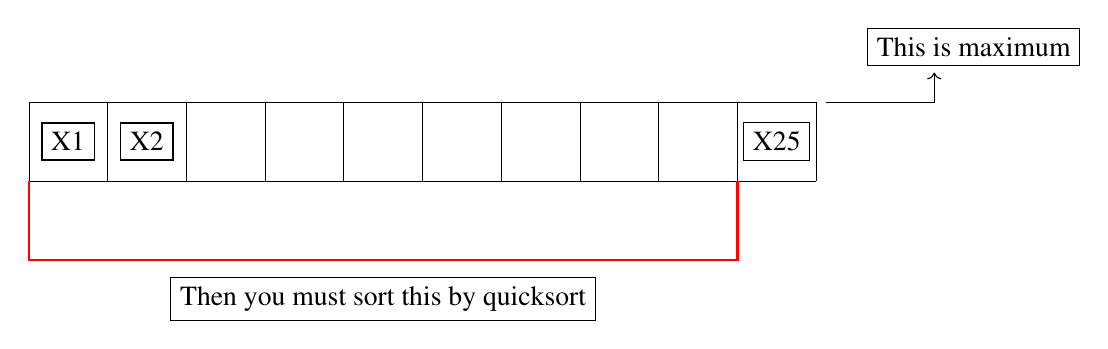
\begin{tikzpicture}
\draw[step=1cm,black,very thin] (0,0) grid (10,1)  node[anchor=north west] {};
\node[draw] at (0.5,0.5) {X1};
\node[draw] at (1.5,0.5) {X2};
\node[draw] at (9.5,0.5) {X25};
\node[draw] at (12,1.7) {This is maximum};
\node[draw] at (4.5,-1.5) {Then you must sort this by quicksort};
\node (A) at (10, 1) {};
\node (B) at (11.5, 1.5) {};
\draw[->, to path={-| (\tikztotarget)}]
  (A) edge (B) ;
\draw[red,thick,solid] (0,0) -- (0,-1) -- (9,-1) -- (9,0);
\end{tikzpicture} 
Minimum, \\ 
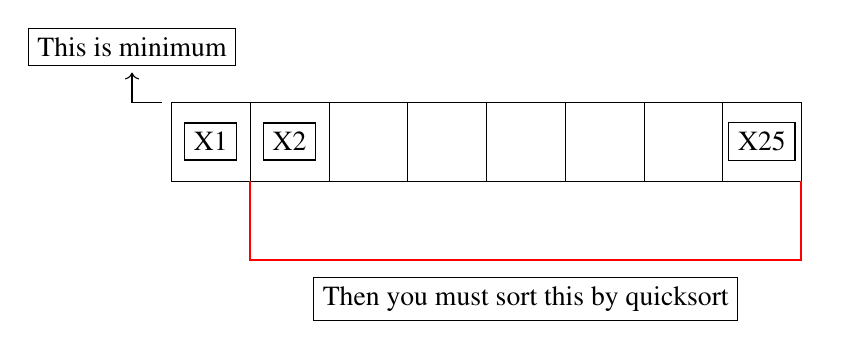
\begin{tikzpicture}
\draw[step=1cm,black,very thin] (0,0) grid (8,1)  node[anchor=north west] {};
\node[draw] at (0.5,0.5) {X1};
\node[draw] at (1.5,0.5) {X2};
\node[draw] at (7.5,0.5) {X25};
\node[draw] at (-0.5,1.7) {This is minimum};
\node[draw] at (4.5,-1.5) {Then you must sort this by quicksort};
\node (A) at (0, 1) {};
\node (B) at (-0.5, 1.5) {};
\draw[->, to path={-| (\tikztotarget)}]
  (A) edge (B) ;
\draw[red,thick,solid] (1,0) -- (1,-1) -- (8,-1) -- (8,0);
\end{tikzpicture}

\end{flushleft}
\end{document}
